\chapter{Metaphor and Coercion} \label{chap:figurative}
In this chapter, I will extend the empirical work on exploring the application of my context sensitive distributional semantic models to two semantic phenomena which involve the application of words in situations where their meanings are in some sense conceptually altered: \emph{metaphor} and \emph{semantic type coercion}.  The precise definitions of these terms, which are not without nuance, was explored in Chapter~\ref{sec:figurative} and will be reintroduced in subsequent sections.  As an overview, the distinguishing characteristic of these phenomena is that they involve cases where what might be thought of as the stable, encyclopedic understanding of some word sense -- a \emph{dictionary definition} of a word, so to speak -- is in some way appropriated or subverted in order to, among other things, transfer information via the attributional conduits connecting figurative source to literal target.

My hypothesis is that, because figurative language always involves the contextual specification of word meaning, context sensitive geometries of lexical representations should provide an appropriate framework for identifying when this type of semantic phenomenon is in effect.  \cite{Fraser1993} demonstrates empirically that metaphor interpretation is, when a metaphor is presented to a subject out of context, an ambiguous exercise, and, to the extent that interpretations of de-contextualised metaphors can be predicted, the predicting factors are themselves culturally relative.  Along similar lines, \cite{BouveretEA2009} propose that metaphor production involves the contextual alignment of overlapping semantic frames, and that this alignment likewise imports structure associated with one frame into the domain of another, evident in, for instance, the additional transposition of syntactic constraints from source to target.  From a cognitive perspective, this coordinates a contextual theory of metaphor with the work on conceptual frames from \cite{Barsalou1992,Barsalou1993} discussed at the end of the previous chapter in the context of judgements of semantic similarity.  From a modelling perspective, this suggests that a methodology for projecting semantic spaces where context specific perspectives can reveal \emph{ad hoc} perspectives on semantic relationships should be a productive approach to identifying figurative language.

The idea that metaphor and metonymy are both instances of ``a connection between two things where one term is substituted for another,'' \citep[][p. 260]{Gibbs1993} will quickly call to mind the premise of distributional semantics: if the motivation for building vector space models of word co-occurrence statistics is that related words have similar co-occurrence tendencies, then figurative language might be construed as a special case in which unrelated or at least conceptually divergent words are likewise found in similar sentential situations.  The question, then, is whether statistical characteristics of the particular co-occurrences profiles selected by words with different meanings are predictive of figurativeness.  A naive hypothesis might be that word combinations that are figurative should simply be further apart in a semantic space than word combination that are literal.  If related words have similar co-occurrence profiles, then maybe unrelated words, for instance words with different conceptual entailments, should have less similar co-occurrence profiles.  This conjecture, however, is belied first of all by the fact that, in the type of corpus containing a broad range of examples of language use necessary for building distributional semantic models, figurative language will already be built into the data (and at the end of this chapter I will argue, in line with, for instance, \cite{Gibbs1994}, that figurative language is going to built into any sample of language no matter how small or basic).  A second problem is that, specifically to overcome the problems with modelling semantic relationships merely in terms of collocations, distributional semantics compares the co-occurrence profiles of words rather than their direct relationships, and it seems likely that word combinations prone to metaphoric interpretation might very well have at least overlapping profiles.

So the objective of the experiments reported in this chapter will be to explore the ways in which and the degrees to which a more fleshed out statistical description of contextually selected distributional semantic subspaces can reveal figurative language.  As with the experiments on relatedness and similarity reported in the previous chapter, in addition to the relationship between target word-vectors in the subspaces they select, the statistical properties of the selected dimensions themselves will also be examined.  And, again as with previous results, the instrument of analysis will be the geometric features of the subspaces in question, with, again, particular attention paid to the way in which the sets of features can collectively indicate figurative language.  The two primary datasets explored represent binary decisions about metaphoricity and coercion respectively, and so my models will be applied to classification tasks here.  In the case of metaphor, I test whether a model learned based on classification data is generalisable to graduated human ratings of metaphoricity.  With the coercion data, I will examine whether the addition of information about sentential context enhances the classification of word pairs.  I will conclude the chapter with a reflection on some of the theoretical implications of the strongly positive results described here.

The study of why humans use figurative language has a considerable scholastic pedigree.

It has served as something of a bafflement to logical empiricists from 

\section{An Experiment on Metaphor}
As pointed out by \cite{ShutovaEA2013}, statistical approaches to metaphor identification and interpretation have generally been formulated in the context of the \emph{conceptual metaphor} theory of \cite{LakoffEA2003}.  This model is founded on the principle that ``we systematically use inference patterns from one conceptual domain to reason about another conceptual domain,'' (ibid, p. 246).  Metaphors are then the mechanism for performing the mapping between these domains, and as such cut right to the core of cognitive processes.  Statistical models of metaphor have accordingly treated metaphors as transformations of lexical representations, and vector space models of distributional semantics have naturally leant themselves to this type of approach.  The construction of representations with the potential to interact with one another in semantically productive ways has in turn lent itself to the development of models that consider the compositional nature of metaphor, effectively treating the metaphor itself as a transformation of the underlying representations.  So \cite{Utsumi2011} constructs candidate metaphor-vectors by calculating the centroid of a number of vectors derived from an analysis of a noun-vector and a predicate-vector learned through latent semantic analysis, and then uses the spatial relationships between these composed vectors to analyse the metaphoricity of certain phrases.  \cite{HovyEA2013} similarly consider composition in their approach to metaphor classification, in this case by combining word-vector type representations with a model trained to identify metaphor based on dependency trees of sentences labelled for metaphoricity.

In the tradition of work on compositional distributional semantics explored by the likes of \cite{MitchellEA2010}, \cite{BaroniEA2010}, and \cite{CoeckeEA2011}, among others, semantic types such as adjectives and verbs are modelled as tensors which perform transformations on nouns, which are modelled as vectors.  In the normal run of things, compositional models therefore represent, for instance, noun phrases modified by adjectives as the product $A\overrightarrow{n}$, where $A$ is a matrix representing an adjective learned from observations of attested instances of the adjective with other noun word-vectors.  So the phrase \emph{black dog} becomes a word-vector in the same space as the representation of just \emph{dog}, and can be compared quantitatively and geometrically with other phrases such as \emph{white dog} or \emph{big cat} and so forth.  In the case of metaphor, these transformations are expected to map the word-vector representing metaphoric phrases into a region corresponding to the semantic domain of the original noun-vector modified by a metaphoric interpretation of the word associated with the tensor of a modifier or a predicate.  So, for instance, in a model that effectively captures metaphoricity, the composition of the vector space representations corresponding to \emph{brilliant light} would map to a region of space where comparisons between phrases like \emph{dark illumination} and \emph{red glow} are productive, while \emph{brilliant child} might be expected to map into the proximity of \emph{stupid boy} and \emph{boring girl}.\footnote{It should be noted that such a methodology at this point begins to assume dim shades of \citepos{Gardenfors2000} conceptual spaces, with different compositions inherently defining different regions of the space.}

The data that I will use in this section to test my methodology was originally presented by \cite{GutierrezEA2016}, along with an accompanying experiment on a novel model.  It consists of 8,592 adjective-noun pairs, spanning 23 adjectives chosen for their membership in six different broad semantic categories that are prone to both literal and metaphoric use: so, for instance, \emph{bitter}, \emph{sour}, and \emph{sweet} are considered constituents of the category \textsc{taste}.  There are also

XXX NOUN-TYPES

Each pair has been rated as either literal or metaphoric by a pair of human annotators, with inter-annotator agreement measuring at Cohen's $\kappa = 0.80$.  This dataset was conceived as something of an expansion of the similar but smaller corpus of adjective-noun phrases annotated with binary metaphoricity classifications presented by \cite{TsvetkovEA2014} (and those authors tested their own data with an assortment of models, achieving highest f-scores by applying a random forest classifier to the features of an existing library of distributional semantic word-vectors).

In their own experimental treatment of the data, \citeauthor{GutierrezEA2016} constructed a pair of compositional models in the mode of \cite{BaroniEA2010}, learning adjective matrixes $A$ to map from noun-vectors to noun-adjective phrase-vectors extracted from observations of co-occurrences of both nouns and phrases in a corpus.  By creating separate tensor representations for literal and metaphoric instances of a given adjective, the authors can then compare the relationships between the vectors resulting from a noun-vector composed with literal and metaphoric senses of an adjective-vector to try to determine whether a given phrase would generally be classified as a metaphor or a literal expression by comparing the respective compared vectors to the phrase-vector as observed in the corpus.  In a further attempt to generalise the method, and, notably, to apply the conceptual metaphor theory of \cite{LakoffEA1980} to their computational model, the authors learn matrices performing linear transformations from literal to metaphoric adjective-noun compositions and then compare the similarity between observed phrase-vectors and literal composed vectors versus transformed literal composed vectors to determine whether a given phrase is metaphoric or not.

The data described by \citeauthor{GutierrezEA2016} will serve as the basis for testing my own context sensitive distributional semantic methodology's ability to classify phrases as literal or metaphoric, and the results of this experiment will be described in the following section.  My hypothesis is that metaphor, and indeed all figurative language, is fundamentally entangled with the context mutually indicated by the representations of the words participating in the composition being analysed.  In fact, I think that part of what is captured by the model described by \citeauthor{GutierrezEA2016}, and indeed a number of other researchers investigating statistical methods for metaphor classification, is precisely that there is a context inherent in the linear algebraic dynamics of composable lexical representations, and this is something which many researchers explicitly recognise.  But I also think that the explicit projection of context specific semantic subspaces, the mainstay of my methodology, should provide an ideal testing ground to discover the way in which statistical geometry can directly broadcast the presence or absence and even potentially the degree of metaphor inherent in a given phrase.  The following sections will test this hypothesis using a similar methodology to that applied to semantic relatedness and similarity in the previous chapter.

%The section after that will explore the geometry of a particularly successful model learned using my methodology.  Finally, in Section~\ref{sec:genafor}, I will address the question of whether a classification model learned from the impressively large dataset contributed by \citeauthor{GutierrezEA2016} can be generalised to handle graduated human ratings of metaphoricity on a different type of metaphoric construction.

\subsection{Methodology and Results}
My own methodology is clearly less committed to maintaining distinct representations for different semantic types than the compositional models described above, instead modelling all words as untagged word-vectors based on their co-occurrences as observed across a large scale corpus.  One motivation for this 

LANGACKER

In this regard, it is more in line with metaphor identifying systems that have used word-vectors consisting of various types of features to, for instance, cluster word senses and then discover metaphorically productive mappings between clusters that are treated as representations of conceptual domains

\begin{table}
\centering
\begin{tabular}{lrrrr|rrrr}
\hline
\emph{window} & \multicolumn{4}{c}{2x2} & \multicolumn{4}{c}{5x5} \\
\emph{dimensions} & 20 & 50 & 200 & \multicolumn{1}{c}{400} & 20 & 50 & 200 & 400 \\
\hline
\textsc{joint} & 0.839 & 0.860 & 0.878 & 0.881 & 0.840 & 0.862 & 0.880 & 0.886 \\
\textsc{indy} & 0.821 & 0.839 & 0.855 & 0.860 & 0.817 & 0.840 & 0.858 & 0.867 \\
\textsc{zipped} & 0.839 & 0.864 & 0.876 & 0.878 & 0.833 & 0.854 & 0.873 & 0.880 \\
\textsc{adjective} & 0.771 & 0.860 & 0.828 & 0.845 & 0.781 & 0.804 & 0.828 & 0.837 \\
\textsc{noun} 0.819 & 0.861 & 0.843 & 0.847 & 0.806 & 0.821 & 0.838 & 0.843 \\
\textsc{SVD} & 0.685 & 0.703 & 0.703 & 0.697 & 0.677 & 0.694 & 0.687 & 0.684 \\
\textsc{SG} & 0.679 & 0.676 & 0.679 & 0.673 & 0.664 & 0.665 & 0.672 & 0.656 \\
\textsc{CBOW} & 0.669 & 0.681 & 0.677 & 0.672 & 0.669 & 0.673 & 0.677 & 0.671 \\
\hline
\end{tabular}
\caption{F-scores for metaphor identification based on a ten-fold cross-validated logistic regression taking geometric features of various subspace types as input.}
\label{tab:related}
\end{table}

Outside of my own methodology, one interesting trend to notice in these results, and in contrast to the results on relatedness and similarity discussed in the previous chapter, is that all three techniques for building static models show an ambiguous trajectory as dimensionality is increased, with in particular a slight but consistent decreases in their agreement with human classifications moving from 200 to 400 dimensional spaces.

As a final point of comparison with other approaches to metaphor classification, I will return briefly to the unannotated character of my lexical representations, mentioned above in the context of

In addition to allowing for a commitment to 

\begin{figure}
  \centering
  \footnotesize
  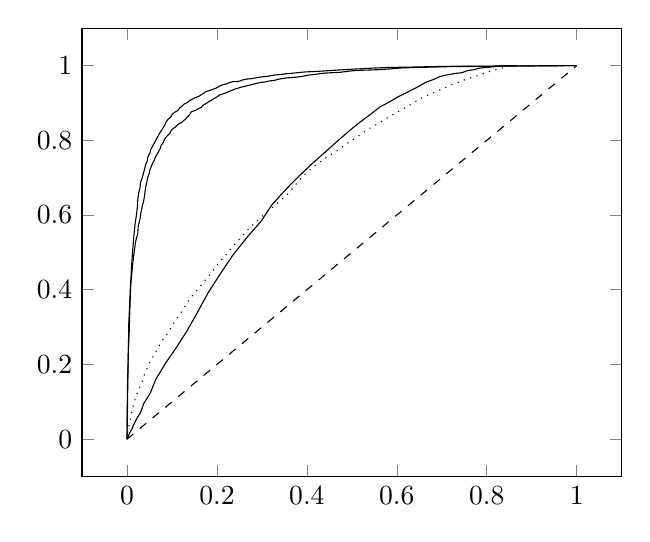
\begin{tikzpicture}
    \begin{axis}[]
      \addplot [dashed] coordinates{(0,0) (1,1)};
      \addplot [] coordinates{(0.0,0.0) (0.001,0.137) (0.003,0.235) (0.004,0.312) (0.006,0.366) (0.008,0.415) (0.010,0.460) (0.012,0.496) (0.014,0.526) (0.016,0.553) (0.018,0.577) (0.021,0.600) (0.023,0.621) (0.024,0.641) (0.026,0.659) (0.029,0.674) (0.030,0.688) (0.034,0.700) (0.037,0.713) (0.039,0.724) (0.042,0.737) (0.045,0.744) (0.046,0.753) (0.048,0.760) (0.051,0.766) (0.052,0.773) (0.056,0.782) (0.059,0.789) (0.062,0.795) (0.064,0.801) (0.067,0.807) (0.070,0.813) (0.073,0.820) (0.076,0.825) (0.080,0.833) (0.082,0.837) (0.084,0.841) (0.086,0.846) (0.088,0.851) (0.091,0.856) (0.094,0.859) (0.098,0.863) (0.099,0.867) (0.102,0.871) (0.106,0.875) (0.109,0.877) (0.113,0.880) (0.115,0.883) (0.117,0.887) (0.121,0.890) (0.125,0.895) (0.127,0.897) (0.131,0.899) (0.134,0.901) (0.137,0.904) (0.140,0.907) (0.143,0.909) (0.147,0.911) (0.151,0.914) (0.156,0.916) (0.160,0.918) (0.164,0.921) (0.166,0.923) (0.170,0.925) (0.173,0.929) (0.178,0.931) (0.183,0.933) (0.187,0.935) (0.192,0.937) (0.197,0.939) (0.203,0.943) (0.209,0.947) (0.214,0.949) (0.221,0.951) (0.229,0.955) (0.236,0.957) (0.244,0.957) (0.252,0.959) (0.258,0.962) (0.267,0.964) (0.277,0.965) (0.290,0.968) (0.301,0.970) (0.310,0.971) (0.320,0.973) (0.330,0.975) (0.341,0.976) (0.352,0.978) (0.363,0.979) (0.379,0.981) (0.396,0.983) (0.413,0.984) (0.430,0.985) (0.455,0.987) (0.483,0.989) (0.511,0.991) (0.543,0.993) (0.582,0.995) (0.632,0.996) (0.709,0.998) (1.0,1.0)}; %joint
      \addplot [thin] coordinates{(0.0,0.0) (0.001,0.084) (0.002,0.171) (0.003,0.238) (0.005,0.291) (0.006,0.333) (0.007,0.370) (0.008,0.409) (0.011,0.447) (0.013,0.474) (0.016,0.501) (0.019,0.528) (0.024,0.551) (0.025,0.571) (0.029,0.590) (0.031,0.607) (0.034,0.624) (0.037,0.638) (0.039,0.651) (0.040,0.663) (0.042,0.677) (0.044,0.688) (0.046,0.700) (0.049,0.710) (0.051,0.721) (0.054,0.730) (0.057,0.739) (0.061,0.748) (0.064,0.757) (0.068,0.765) (0.071,0.772) (0.074,0.778) (0.076,0.787) (0.080,0.793) (0.083,0.802) (0.086,0.807) (0.091,0.814) (0.095,0.818) (0.098,0.826) (0.102,0.831) (0.107,0.835) (0.111,0.840) (0.116,0.845) (0.122,0.848) (0.126,0.853) (0.130,0.856) (0.133,0.861) (0.136,0.864) (0.140,0.870) (0.143,0.876) (0.149,0.879) (0.154,0.881) (0.159,0.885) (0.165,0.888) (0.169,0.894) (0.174,0.897) (0.180,0.902) (0.184,0.905) (0.188,0.907) (0.192,0.911) (0.197,0.914) (0.201,0.917) (0.205,0.921) (0.210,0.923) (0.215,0.925) (0.220,0.927) (0.227,0.931) (0.234,0.934) (0.242,0.938) (0.248,0.940) (0.253,0.942) (0.261,0.944) (0.267,0.946) (0.274,0.948) (0.281,0.950) (0.290,0.953) (0.297,0.955) (0.307,0.956) (0.317,0.959) (0.327,0.960) (0.335,0.963) (0.344,0.965) (0.354,0.967) (0.366,0.968) (0.376,0.969) (0.389,0.971) (0.400,0.974) (0.415,0.976) (0.427,0.978) (0.441,0.980) (0.456,0.981) (0.474,0.982) (0.493,0.985) (0.510,0.987) (0.535,0.988) (0.558,0.989) (0.584,0.991) (0.614,0.994) (0.649,0.995) (0.708,0.997) (1.0,1.0)}; %indy
      \addplot [dotted] coordinates {(0.000,0.000) (0.000,0.000) (0.000,0.000) (0.000,0.000) (0.000,0.000) (0.000,0.000) (0.000,0.000) (0.000,0.000) (0.000,0.000) (0.000,0.000) (0.000,0.000) (0.000,0.000) (0.000,0.000) (0.000,0.000) (0.000,0.000) (0.000,0.002) (0.000,0.003) (0.000,0.006) (0.000,0.009) (0.001,0.013) (0.001,0.020) (0.003,0.029) (0.005,0.040) (0.008,0.055) (0.010,0.070) (0.014,0.090) (0.019,0.110) (0.025,0.131) (0.034,0.155) (0.041,0.180) (0.051,0.206) (0.063,0.232) (0.076,0.260) (0.090,0.283) (0.104,0.311) (0.121,0.341) (0.140,0.376) (0.159,0.404) (0.180,0.434) (0.200,0.466) (0.221,0.495) (0.243,0.526) (0.264,0.555) (0.285,0.580) (0.309,0.606) (0.332,0.629) (0.356,0.654) (0.376,0.683) (0.396,0.710) (0.418,0.732) (0.442,0.753) (0.469,0.774) (0.490,0.792) (0.514,0.811) (0.535,0.829) (0.559,0.845) (0.580,0.861) (0.600,0.875) (0.618,0.887) (0.638,0.901) (0.656,0.914) (0.672,0.922) (0.690,0.932) (0.708,0.941) (0.723,0.950) (0.739,0.956) (0.753,0.963) (0.766,0.968) (0.777,0.972) (0.786,0.976) (0.796,0.980) (0.806,0.984) (0.816,0.988) (0.825,0.991) (0.833,0.993) (0.839,0.995) (0.843,0.997) (0.848,0.999) (0.854,0.999) (0.857,0.999) (0.861,1.000) (0.864,1.000) (0.867,1.000) (0.868,1.000) (0.869,1.000) (0.869,1.000) (0.869,1.000) (0.869,1.000) (0.869,1.000) (0.869,1.000) (0.869,1.000) (0.869,1.000) (0.869,1.000) (0.869,1.000) (0.869,1.000) (0.869,1.000) (0.869,1.000) (0.869,1.000) (0.869,1.000) (1.0,1.0)}; %cbow, auc = 0.722
      \addplot [] coordinates{(0.000,0.000) (0.000,0.000) (0.000,0.000) (0.000,0.000) (0.000,0.000) (0.000,0.000) (0.000,0.000) (0.000,0.000) (0.000,0.000) (0.000,0.000) (0.000,0.000) (0.000,0.000) (0.000,0.000) (0.000,0.000) (0.000,0.000) (0.000,0.000) (0.000,0.000) (0.000,0.000) (0.000,0.000) (0.000,0.000) (0.000,0.000) (0.000,0.001) (0.001,0.002) (0.001,0.003) (0.002,0.005) (0.003,0.009) (0.005,0.014) (0.007,0.020) (0.011,0.027) (0.015,0.039) (0.022,0.056) (0.030,0.071) (0.037,0.095) (0.052,0.124) (0.064,0.160) (0.086,0.204) (0.109,0.244) (0.134,0.291) (0.156,0.338) (0.180,0.391) (0.206,0.440) (0.235,0.492) (0.266,0.539) (0.298,0.583) (0.322,0.627) (0.352,0.667) (0.383,0.705) (0.414,0.740) (0.444,0.772) (0.468,0.798) (0.492,0.823) (0.515,0.846) (0.540,0.868) (0.562,0.889) (0.584,0.903) (0.605,0.918) (0.627,0.931) (0.645,0.942) (0.664,0.955) (0.682,0.963) (0.696,0.971) (0.712,0.975) (0.730,0.979) (0.745,0.981) (0.758,0.987) (0.772,0.989) (0.780,0.992) (0.790,0.994) (0.800,0.995) (0.808,0.996) (0.816,0.997) (0.822,0.998) (0.828,0.999) (0.835,0.999) (0.838,1.000) (0.843,1.000) (0.847,1.000) (0.852,1.000) (0.857,1.000) (0.862,1.000) (0.864,1.000) (0.866,1.000) (0.867,1.000) (0.868,1.000) (0.868,1.000) (0.868,1.000) (0.868,1.000) (0.868,1.000) (0.868,1.000) (0.868,1.000) (0.868,1.000) (0.868,1.000) (0.868,1.000) (0.868,1.000) (0.868,1.000) (0.868,1.000) (0.868,1.000) (0.868,1.000) (0.868,1.000)}; %svd 2x50, auc = 0.720
    \end{axis}
  \end{tikzpicture}
\caption{Receiver operator characteristic plots for a selection of models, with the area under the curve for each model type indicated in the legend.}
\label{fig:meanmax}
\end{figure}

\subsection{The Geometry of Metaphor}
\begin{table}
\centering
\begin{tabular}{lr|lr|lr|lr|lr}
\hline
\multicolumn{2}{c}{\textsc{joint}} & \multicolumn{2}{c}{\textsc{indy}} & \multicolumn{2}{c}{\textsc{zipped}} & \multicolumn{2}{c}{\textsc{adjective}} & \multicolumn{2}{c}{\textsc{noun}} \\
\hline
$\mu(A,B)$ & 0.787 & $C$ & 0.767 & $\mu(A,B)$ & 0.788 & $\mu(A,B)/M$ & 0.745 & $\mu(A,B)$ & 0.756 \\
$C$ & 0.771 & $C/M$ & 0.749 & $C$ & 0.771 & $\overline{AC}:\overline{BC}$ & 0.736 & $C$ & 0.747 \\
$\mu(A,B)/M$ & 0.764 & $\angle AMB$ & 0.747 & $\mu(A,B)/M$ & 0.769 & $\overline{AC}/\overline{BC}$ & 0.734 & $\mu(A,B)/X$ & 0.728 \\
$\angle COX$ & 0.762 & $C/X$ & 0.746 $X$ & 0.767 & $\mu(A,B)/X$ & 0.732 & $\mu(A,B)/M$ & 0.721 \\
$X$ & 0.762 & $\mu(A,B)$ & 0.734 & $\mu(A,B)/X$ & 0.759 & $\angle ACB$ & 0.730 & $C/X$ & 0.721 \\
\hline
\end{tabular}
\caption{Independent f-scores from the metaphor classification data for top five features of each subspace type for 5x5 word co-occurrence window, 400 dimension subspaces.}
\label{tab:ind-metaphor}
\end{table}

\subsection{Generalising the Model} \label{sec:genaphor}
One of the interesting things about feature-based classification is that there is always an inherent commitment to degree of class membership, even when the training data used to build a model is simply binary.  This is true of any model which uses, for instance, a logistic regression technique for determining class, as there is a cut-off point along the spectrum of model output and a corresponding proximity to that point for any given sample, and it is especially obvious when the features of the model are actually geometrical measures.  In this section, I will apply the models learned from the the \cite{GutierrezEA2016} data to another dataset designed to assess metaphor as a matter of degree rather than simply as a binary situation

\section{An Experiment on Coercion}

\subsection{Methodology and Results}

\subsection{The Geometry of Coercion}

\subsection{Adding Sentential Context}

\section{Interpretation and Composition in Context}

In fact, it is tempting to go so far as to say that figurative language is identified precisely as those instances of language where recourse to a conceptual context is necessary to interpret a lexical composition, and furthermore that the degree of figurativeness correlates with the extent of context construction involved in an interpretation.  This proposition is in line with \citepos{Shutova2015} empirical work treating metaphor interpretation as a mechanism for classification

This, then, raises a valid question: is the role of figurative language exclusively, or even for that matter primarily, to port attributes from one conceptual domain to another?  Or is what metaphor does, as \cite{Davidson} has famously suggested, really about something more fundamentally phenomenological than just the efficient transmission of propositions?  So, where, for instance, \cite{Sweetser} sees polysemy as an intermediate stage bridging the progress from literal to metaphoric usage, my methodology leaves itself open to the possibility that all usage is, in fact, first and foremost pragmatic, and only secondarily lexicalised.  By this interpretation, words have semantic affordances in terms of their potential to convey cognitive content intersubjectively, and they are picked up and used in much the same way that a cognitive agent might adapt an object designed or just perceived as being for one purpose as an implement in another activity---using a shoe as a hammer, for example, or a chair to fend off a lion.  The cognitive foregrounding of this nascent theory can be found in the ecological psychology of \cite{Gibson} and \cite{Bateson}, and the linguistic correlary seems to be in line with what psycholinguists inspired by biosemiotics such as \cite{Raczsek} are saying about the way that language is primarily about affording cognitive value to interlocutors, including but hardly limited to truth values.

This theoretical speculation is a potential extrapolation of my methodology rather than a precondition for it, and is offered primarily as an example of how this statistical approach might become a component of productive line of philosophical enquiry.  The point, though, is that with a geometric methodology, relationships between lexical semantic representations can be recast as Gibsonian affordances: there is a mechanism for the direct perception of opportunities for meaning making in the actual layout of the statistical environment
